The main goal of this chapter is giving an overview of the definitions in literature of the term "visualization". Visualization is first mentioned but not defined in 1953 in cartographic literature, in an article by University of Chicago geographer Allen K. Philbrick. \citeauthor{mccormick:1987} took up the term and defined it as follows:
\begin{quote}
 "Visualization is a method of computing. It transforms the symbolic into the geometric, enabling researchers to observe their simulations and computations. Visualization offers a method for seeing the unseen. It enriches the process of scientific discovery and fosters profound and unexpected insights. In many fields it is already revolutionizing the way scientists do science.

 Visualization embraces both image understanding and image synthesis. That is, visualization is a tool for both for interpreting image data fed into a computer, and for generating images from complex multi-dimensional data sets. It studies those mechanisms in humans and computers which allow them in concert to preceive, use and communicate visual information \iacite{mccormick:1987}."
\end{quote}

In 1987, new developments in the field of computer science prompted the National Science Foundation to redefine the term. The report of the redefinition placed visualization at the convergence of computer graphics, image processing, computer vision, computer-aided design, signal processing, and user interface studies \iacite{mccormick:1987}. \citeauthor{Phillips2010} discuss three elemental issues existing today in the research field of visualization:

\begin{enumerate}
\item to settle on a definition for the term "visualization"
\item to clarify the underlying presumptions and
\item to decide how to document both short-term and long-term effectiveness.
\end{enumerate}

\begin{quote}
The status of terms, often used interchangeably, such as "visualization", "visual representation", "visual media", "media literacy", "visual communication skills", "visual literacy", "illustrations", and "media illustrations", is yet to be clarified. Furthermore, the routine confusion between pictures/visual images and reality is a fundamental and persistent problem \iacite{Phillips2010}.
\end{quote}

Because of the wide reach of the term, \citeauthor{Phillips2010} use a series of five steps in order to tell how "visualization" is defined in literature. The steps can be summarized as follows:
\begin{enumerate}
\item A search of all relevant sources, the identification of vocabulary and the mapping of the citations.
\item Classify the types of research into explanatory, exploratory, descriptive studies and "other".
\item Analyse and evaluate the assertions made in step two.
\item Organization of the reviews through comparisons of the literature, in order to identify areas of difference and similarity.
\item Mapping the collected information on several categories.
\end{enumerate}
The evaluation of this method used a total of 247 articles, ranging from the year 1936 to 2009. Out of those articles, 56\% were empirical studies and 44\% discussion articles. Figure \ref{fig:evaluation-definition} on page \pageref{fig:evaluation-definition} shows, that all articles have been organized by subject area.

\begin{figure}[!htb]
\centering
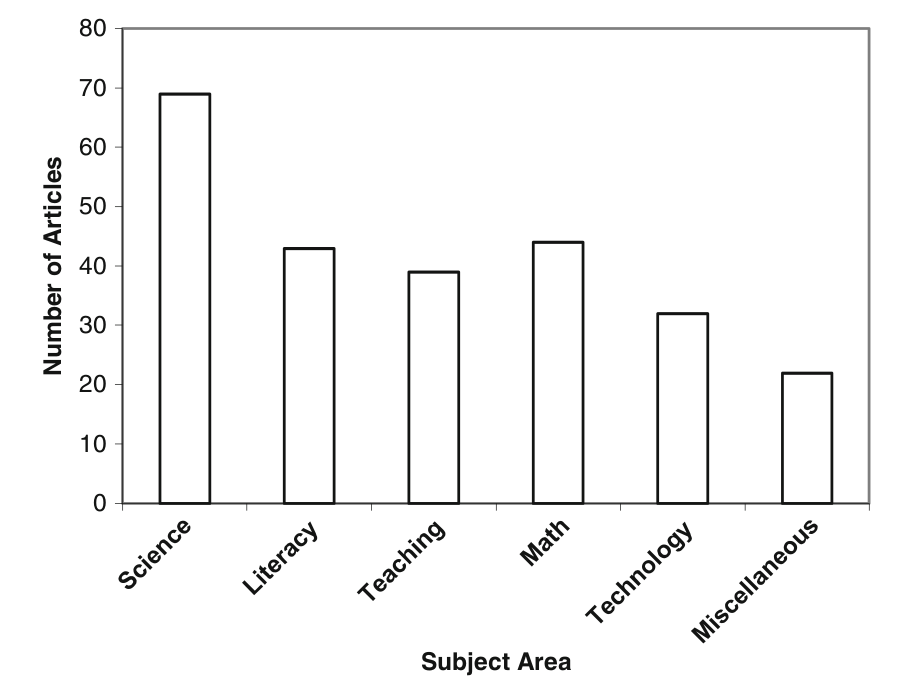
\includegraphics[width=0.8\textwidth,keepaspectratio]{images/definition/evaluation-definition.png}
\caption[
    The number of published articles organized by subject area \iacite{Phillips2010}.
]{The number of published articles organized by subject area.}
\label{fig:evaluation-definition}
\end{figure}

\citeauthor{Phillips2010} found out, that the attempt to define "visualization" in literature is not possible. The term is substituted frequently with terms like "visual aid", "image", "visual literacy" etc.

To clarify the term with a relation to the progress made the last years, two well known online dictionaries are used. One possible generic definition could be the one from Oxford Dictionaries\footnote{See \href{https://www.oxforddictionaries.com/definition/english/visualization}{Oxford Dictionaries}}:

\begin{quote}
\begin{enumerate}
\item "The representation of an object, situation, or set of information as a chart or other image."
\item "The formation of a mental image of something."
\end{enumerate}
\end{quote}

Even though the noun "visualization" has a very close related verb, \citeauthor{Phillips2010} noted the important distiction between those. The noun "[\ldots] directs the attention to the product, the object, the 'what' of visualization, the visual images. The verb of visualization on the other hand makes one attend to the process, the activity, the skill, the 'how' of visualizing" \iacite{Phillips2010}.

Another possible definition for "visualization" is represented in table \ref{tab:meriam-dict} on page \pageref{tab:meriam-dict}. It contains a specification of the meanings found from the Merriam Webster Online Dictionary\footnote{\label{mod}See \href{http://www.merriam-webster.com/}{Merriam Webster Dictionary}}.

\begin{table}[!htp]
\centering
\begin{tabular}{l p{10cm}}

%row
Visualization (noun) &

\begin{enumerate}[leftmargin=*]
\item formation of mental images
\item act or process of interperting in visual terms or of putting into visible form
\end{enumerate}
\\[4ex]


%row
Visualize (transitive verb) &
To make visible: as to see or form a mental image of
\\[4ex]


%row
Image (noun) &
\begin{enumerate}[leftmargin=*]
\item a reproduction or imitation of the form of a person or thing
\item
    \begin{enumerate}
    \item the optical counterpart of an object produced by an optical device (as a lens or mirror) or an electronic device
    \item a visual representation of something: a likeness of an object produced on a photographic material, or a picture produced on an electronic display (as a television or computer screen)
    \end{enumerate}
\item a tangible or visible representation
\item a mental picture or impression of something
\item a vivid or graphic representation or description
\end{enumerate}
\\[4ex]

%row
Image (transitive verb) &
\begin{enumerate}[leftmargin=*]
\item to call up a mental picture
\item to describe or portray in language especially in a vivid manner
\item to create a representation
\end{enumerate}
\\[4ex]


%row
Visual literacy (noun) &
the ability to recognize and understand ideas conveyed through visible actions or images (as pictures)

\end{tabular}
\caption[
Definitions of terms from Merriam-Webster Online Dictionary, Urldate: 07.2016
    \newline\small\texttt{\url{http://www.merriam-webster.com/}}
]{Definitions of terms from Merriam-Webster Online Dictionary}
\label{tab:meriam-dict}
\end{table}

Combining the already mentioned definitions of terms with the research results from \citeauthor{Phillips2010},a three-fold distinction of definitions is visible:
\begin{enumerate}
\item Physical objects serving as visualizations (e.g. geometrical illustrations). These objects are viewed and interpreted by a person for the purpose of understanding something.
\item Mental objects pictured in the mind (e.g. mental imagery). These are imaginative constructions of some possible visual experiences.
\item Cognitive processing in which visualizations are interpreted, either physical or mental (e.g. cognitive manipulation of visual representations by the mind). This often refers as an act of deriving meaning from a physical or mental object.
\end{enumerate}

According to \citeauthor{Phillips2010} the distinction between physical and mental visualization objects are obvious. This statement is also verified by the given definition of \citeauthor{mccormick:1987} where this exact distinction is already made. However the distinction between the visualization itself and the thinking involved in interpreting it is also important \iacite{Phillips2010}.